\documentclass[11pt]{report}
\usepackage[a4paper, top=3cm, bottom=3cm]{geometry}

\usepackage[dutch]{babel}
\selectlanguage{dutch}

\usepackage{color}
\definecolor{gray75}{gray}{0.75}

\usepackage{framed}

\usepackage{graphicx}
\usepackage{tikz}

\usepackage{amsmath}

\usepackage[colorlinks=true,linkcolor=black]{hyperref}

\usepackage[T1]{fontenc}
\usepackage{titlesec}

\newcommand{\hsp}{\hspace{15pt}}

\titleformat{\chapter}[hang]{\Huge\bfseries}{\thechapter\hsp\textcolor{gray75}{|}\hsp}{0pt}{\Huge\bfseries}
\titlespacing{\chapter}{0pt}{-3.5ex plus 1ex minus .2ex}{2.3em plus .2ex}

\newlength{\leftbarwidth}
\setlength{\leftbarwidth}{3pt}
\newlength{\leftbarsep}
\setlength{\leftbarsep}{10pt}

\newcommand*{\leftbarcolorcmd}{\color{leftbarcolor}}% as a command to be more flexible
\colorlet{leftbarcolor}{black}

\renewenvironment{leftbar}{%
    \def\FrameCommand{{\leftbarcolorcmd{\vrule width \leftbarwidth\relax\hspace {\leftbarsep}}}}%
    \MakeFramed {\advance \hsize -\width \FrameRestore }}{\endMakeFramed}

\begin{document}

\begin{titlepage}
\begin{center}
{\huge\bfseries A New Field-Effect Transistor with Selectively Doped $GaAs/n-Al_{x}Ga_{1-x}As$ Heterojunction}
\\ \bigskip
{\Large Discussie \& kwalitatieve analyse}
\end{center}
\vfill
\begin{flushleft}
\setlength{\leftbarwidth}{1pt}
\colorlet{leftbarcolor}{gray75}
\begin{leftbar}
Halfgeleiders \\
Jelle Verstraaten, 500236946 \\
\texttt{jelle@benext.nl} \\
Erik Steuten\\
E-technology \\
{\small \today} \\
\end{leftbar}
\end{flushleft}
\end{titlepage}

\tableofcontents
%\listoffigures
%\listoftables

\chapter{Inleiding}
%In dit hoofdstuk wordt ingegaan op de de schrijvers van het artikel, het onderzoeklaboratorium waar zij werkten en het artikel in het algemeen.

Het artikel dat behandeld wordt, ``A New Field-Effect Transistor with Selectively Doped $GaAs/n-Al_{x}Ga_{1-x}As$ Heterojunction'', is geschreven door Takashi Mimura, Satoshi Hiyamizu, Toshio Fuji en Kazuo Nanbu in 1980. Het artikel is gepubliceerd in het Japanese Journal of Applied Physics (JJAP). Alle artikelen in dit paper zijn gepeer-reviewed. Het artikel borduurd voort een artikel an Dingle et al (Bell Laboratories): ``Electron mobilities in modulation-doped semiconductor heterojunction superlattices''.

Het artikel is gepubliceerd dit in opdracht van Fujitsu Laboratories Ltd. Fujitsu was ge\"interesseerd in het vercommercializeren van de ontdekking die gedaan is door Dingle. Nadat Dingle zijn onderzoek had gepubliceerd ontstond er namelijk een ware race om de eerste te zijn die deze technologie werkend te krijgen.

Er is een patent van Daniel Delagebeaudeuf en Trong L Nuyen, ``Field effect transistor with a high cut-off frequency ''. Dit patent borduurd voort op het werk van Mimura et al. en Dingle et al. Beide waren werkzaam bij Thomson-CSF. Dit lab was in staat waren een betere variant van de transistor te fabriceren. 

De abstract is duidelijk om geeft meteen aan waarom dit nieuwe type FET interessant is. De reden is dat deze FET veel (tot 3x) hogere frequenties aankan dan de huidige ontwerpen. 

In de inleiding wordt duidelijk gemaakt dat dit artikel voortborduurt op het artikel van Dingle et al. In dit artikel wordt een nieuw fenomeen gerapporteerd, namelijk de hogere mobiliteit van elektronen in AlGaAs/GaAs heterojunction. In dit artikel wordt verder gegaan met deze ontdekking en wordt gekeken hoe deze hogere mobiliteit gebruikt kan worden in nieuwe halfgeleider componenten. Deze inleiding geeft een goed beeld van de context waarin het artikel geschreven is.

\chapter{Discussie}
De hoofdvraag van dit artikel is: ``Kan de hogere elektronmobiliteit van een heterojunction gebruikt worden voor het fabriceren van een snellere transistor?''. Deze hoofdvraag wordt experimenteel bevestigd door het cree\"eren van onder andere transistoren, diodes en hall-bruggen en het testen hiervan.

De resultaten van de testen bevestigen de voorgaande bevindingen van Dingle et al. en wijzen erop dat er een 2-dimensionaal elektrongas ontstaat. Ook wordt aangetoond dat het mogelijk is om het elektrongas te moduleren door het drain-voltage $V_{DS}$ op de transistor te vari\"eren. Deze resultaten zijn belangrijk omdat hiermee de onderzoeksvraag beantwoord kan worden. Ook kan uit deze resultaten afgeleid worden dat dit nieuwe transistorontwerp, op hoge frequenties, inderdaad beter werkt dan andere ontwerpen.

%  - Hoe goed waren de methodes die in het onderzoek zijn gebruikt?

\chapter{Resultaten}
\section{Figuur 1}
\begin{figure}[h]
\centering
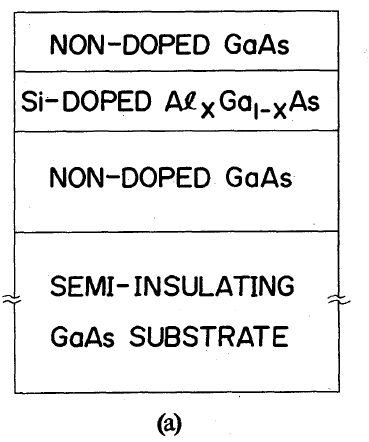
\includegraphics[width=0.5\textwidth]{physical_structure.png}
\caption{}
%\label{fig:}
\end{figure}

\section{Figuur 2}
\begin{figure}
\centering
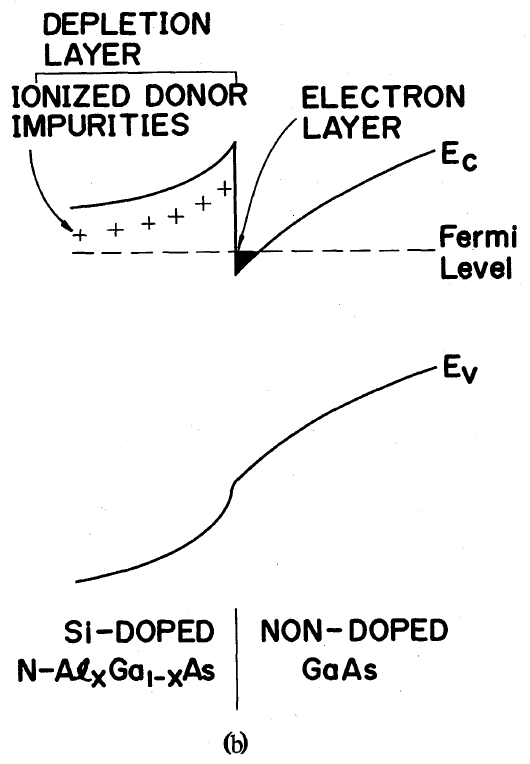
\includegraphics[width=0.5\textwidth]{bandenergy_structure.png}
\caption{}
%\label{fig:}
\end{figure}

\section{Figuur 3}
\begin{figure}
\centering
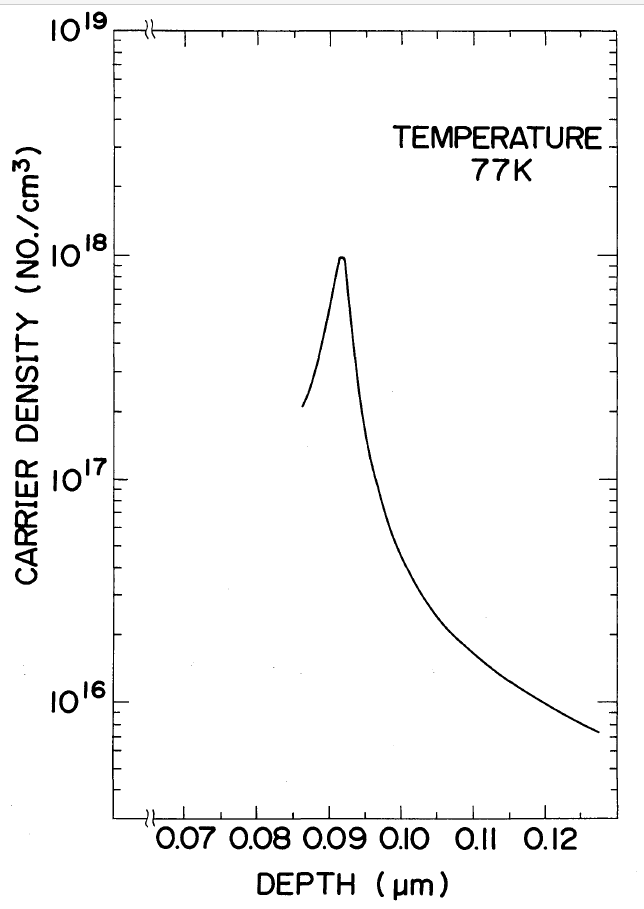
\includegraphics[width=0.5\textwidth]{carrier_profile_depth.png}
\caption{}
%\label{fig:}
\end{figure}

\section{Figuur 4}
\begin{figure}
\centering
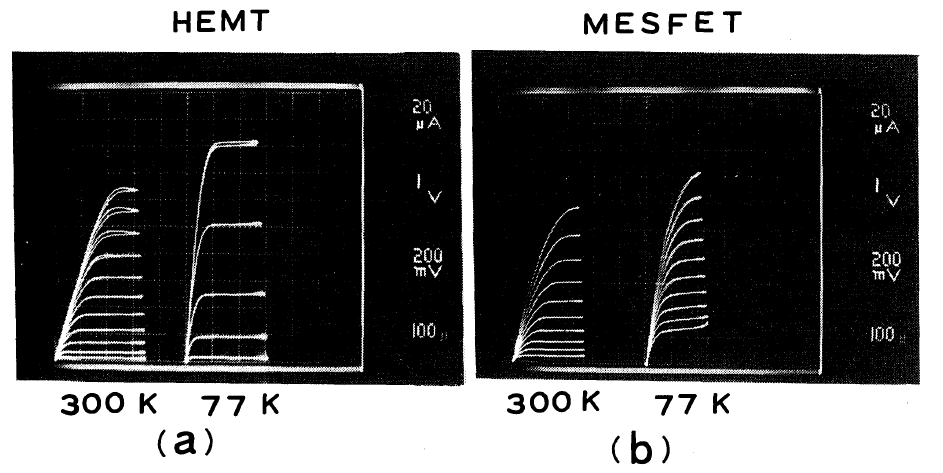
\includegraphics[width=0.5\textwidth]{CV-characteristics.png}
\caption{}
%\label{fig:}
\end{figure}

  - Gedetaileerde beschrijving van de resultatenin tabellen, figuren, etc.
  - Laat zien waar je dit terugvindt in het artikel

\chapter{Experimenten}
  - Welke opstellingen zijn er gebruikt?
  - Welke methoden zijn er gebruikt?

\chapter{Referenties}
  - Welke methode wordt gebruikt om referenties weer te geven?
  - Zoek de referentie waarnaar het artikel het meeste refereert, voeg een kopie toe

\bibliographystyle{IEEEtran}
\bibliography{literatuur/literature}

\appendix

\end{document}

Electron mobilities in modulation‐doped semiconductor heterojunction superlattices

%Verslag
%- Over het artikel
%- Goed lopend verhaal
%- Hoe lang moet het verslag zijn?
%- Voeg een kopie van het artikel toe
%- Voeg een kopie toe van het artikel waarnaar het meeste gerefereert wordt.
%- Analoge EN digitale kopie

%Inleverdatum: 2015-06-22
%Herkansing: 2015-08-31
